\chapter{Corriente resistencia y fuerza electromotriz}
Una \textit{corriente eléctrica} consiste en cargas en movimiento de una región a otra. Cuando este desplazamiento tiene lugar en una trayectoria de conducción que forma una espira cerrada, la trayectoria recibe el nombre de \textit{circuito eléctrico}, los cuales, fundamentalmente, son un medio de transportar \textit{energía} de un lugar a otro.

\section{Corriente eléctrica}
Una \textbf{corriente eléctrica} es todo movimiento de carga de una región a otra.

\subsection{Dirección del flujo de corriente}
Definimos que la corriente, denotada por $I$, va en la dirección en la que hay un flujo de carga \textit{positiva}.  Por ello, las corrientes se describen como si consistieran por completo en un flujo de cargas positivas, aun en los casos en que se sabe que la corriente real se debe a electrones. Esta convención sobre la dirección del flujo de la corriente se llama \textbf{corriente convencional}. Aunque la dirección de la corriente convencional \textit{no} es necesariamente la misma en que se desplazan en realidad las partículas con carga. Definimos la corriente a través del área de sección transversal $A$ como la carga neta que fluye a través del área por unidad de tiempo. De esta forma, si una carga neta $dQ$ fluye a través de un área en el tiempo $dt$, la corriente $I$ a través del área es

\begin{equation}\label{25.1}\marginnote{Definición de corriente}
I=\frac{dQ}{dt}
\end{equation}

\textbf{La corriente no es un vector}.

La unidad del SI para la corriente es el \textbf{ampere}.

\subsection{Corriente, velocidad de deriva y densidad de corriente}

\begin{figure}[h]
\centering
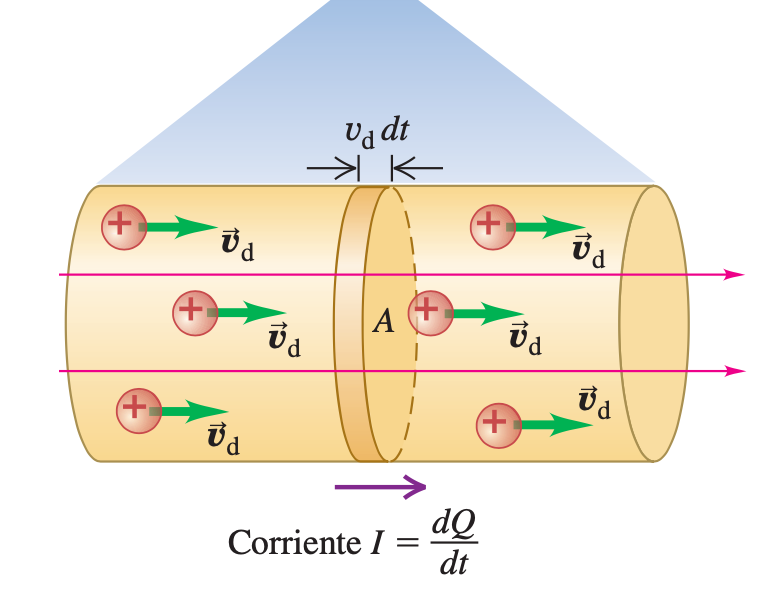
\includegraphics[scale=0.4]{fig/corriente}
\caption{La corriente $I$ es la tasa de transferencia de carga a través del área de la sección transversal $A$. La corriente va en la misma dirección de $\vec{E}$ sin que importe si las cargas en movimiento son positivas}
\label{fig:corriente}
\end{figure}

La corriente se puede expresar en términos de la velocidad de deriva de las cargas en movimiento. Consideremos la situación de la figura \ref{fig:corriente}. Suponga que hay $n$ partículas con carga en movimiento por unidad de volumen. Llamaremos $n$ a la concentración de partículas. Suponemos que todas las partículas se mueven con la misma velocidad de deriva con magnitud $v_d$. En un intervalo de tiempo $dt$, cada partícula se mueve una distancia $v_d\, dt$. Las partículas que fluyen hacia fuera del extremo derecho del cilindro sombreado cuya longitud es $v_d\, dt$ durante $dt$ son partículas que estuvieron dentro del cilindro al comienzo del intervalo $dt$. El volumen del cilindro es $Av_d\, dt$, y el número de partículas dentro es $nAv_d\, dt$. Si cada partícula tiene una carga $q$, la carga $dQ$ que fluye hacia fuera por el extremo del cilindro durante el tiempo $dt$ es

\begin{equation*}
dQ=q(nAv_d\, dt) = nqv_dA\, dt
\end{equation*}

y la corriente es

\begin{equation*}
I=\frac{dQ}{dt}=nqv_dA
\end{equation*}

La \textit{corriente por unidad de área de la sección transversal} se denomina \textbf{densidad de corriente} $J$:

\begin{equation*}
J=\frac{I}{A}=nqv_d
\end{equation*}

Si las cargas en movimiento son negativas en vez de positivas, la velocidad de deriva es opuesta a $\vec{E}$. Pero la corriente aún tiene la misma dirección que $\vec{E}$ en cada punto del conductor. Entonces, la corriente $I$ y la densidad de corriente $J$ no dependen del signo de la carga, por lo que en las expresiones anteriores para $I$ y $J$, la carga $q$ se sustituye por su valor absoluto $|q|$:

\begin{equation}\label{25.2}\marginnote{Expresión general para la corriente}
\boxed{I=\frac{dQ}{dt}=n|q|v_dA}
\end{equation}

\begin{equation}\label{25.3}\marginnote{Expresión general para la densidad de corriente}
J=\frac{I}{A}=n|q|v_d
\end{equation}

Se puede definir además una densidad de corriente vectorial $\vec{J}$ que incluye la dirección de la velocidad de deriva:

\begin{equation}\label{25.4}\marginnote{Densidad de corriente vectorial}
\boxed{\vec{J}=nq\vec{v}_d}
\end{equation}

Es posible tener una corriente \textit{estacionaria}, es decir, constante en el tiempo, sólo si el material conductor forma una espira cerrada, llamada \textit{circuito completo}. En una situación estacionaria, la carga total en cada segmento del conductor es constante. Por lo tanto, la tasa de flujo de carga hacia fuera de un extremo de un segmento en cualquier instante es igual a la tasa de flujo de carga hacia dentro en el otro extremo del segmento, y \textit{la corriente es la misma en todas las secciones transversales del circuito}.

\section{Resistividad}
La \textbf{resistividad} $\rho$ de un material se define como la razón de las magnitudes del campo eléctrico y la densidad de corriente:

\begin{equation}\label{25.5}\marginnote{Definición de resistividad}
\boxed{\rho=\frac{E}{J}}
\end{equation}

Un conductor perfecto tendría una resistividad igual a cero; y un aislante perfecto tendría resistividad infinita.

El recíproco de la resistividad es la \textbf{conductividad}.

Un material que obedece razonablemente bien la ley de Ohm se llama conductor \textit{óhmico} o \textit{conductor lineal}. 

\section{Resistencia}

\begin{figure}[h]
\centering
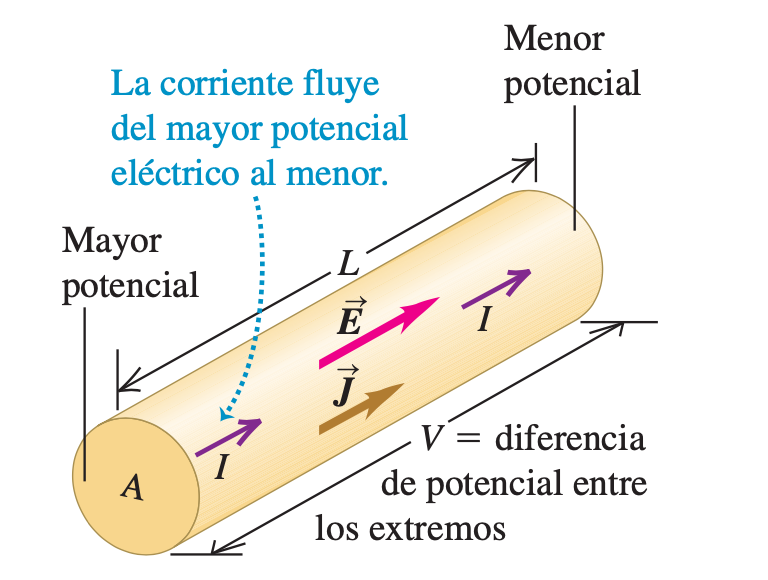
\includegraphics[scale=0.4]{fig/resistencia}
\caption{Conductor con sección transversal uniforme. La densidad de corriente es uniforme sobre cualquier sección transversal, y el campo eléctrico es constante en toda la longitud.}
\label{fig:resistencia}
\end{figure}

Para un conductor con resistividad $\rho$, con densidad de corriente $\vec{J}$ en un punto, el campo eléctrico $\vec{E}$ está dado por la ecuación \ref{25.5}

\begin{equation}\label{25.7}
 \vec{E}=\rho\vec{J}
\end{equation}

Suponga que nuestro conductor es un alambre con sección transversal uniforme de área $A$ y longitud $L$, como se ilustra en la figura \ref{fig:resistencia}. Sea $V$ la diferencia de potencial entre los extremos de mayor y menor potencial del conductor, de manera que $V$ es positiva. La \textit{dirección} de la corriente siempre va del extremo de mayor potencial al de menir potencial. Esto se debe a que en un conductor la corriente fluye en dirección de $\vec{E}$, sin importar el signo de las cargas en movimiento, y porque $\vec{E}$ apunta en la dirección del potencial eléctrico \textit{decreciente}.

También se puede relacionar el \textit{valor} de la corriente $I$ con la diferencia de potencial entre los extremos del conductor. Si las magnitudes de la densidad de corriente $\vec{J}$ y el campo eléctrico $\vec{E}$ son uniformes a través del conductor, la corriente total $I$ está dada por $I=JA$, y la diferencia de potencial $V$ entre los extremos es $V = EL$. Cuando se despejan $J$ y $E$, respectivamente, en estas ecuaciones y se sustituyen los resultados en la ecuación \ref{25.7}, se obtiene lo siguiente:

\begin{equation}\label{25.8}
\frac{V}{L}=\frac{\rho I}{A} \qquad \textup{o bien,}\qquad  V=\frac{\rho L}{A}I
\end{equation}

La razón de $V$ a $I$ para un conductor particular se llama \textbf{resistencia}, $R$:

\begin{equation}\label{25.9}
R=\frac{V}{I}
\end{equation}

Al comparar esta definición de $R$ con la ecuación \ref{25.8}, se observa que la resistencia $R$ de un conductor particular se relaciona con la resistividad $\rho$ del material mediante la ecuación

\begin{equation}\label{25.10}\marginnote{Relación entre la resistencia y la resistividad}
R=\frac{\rho L}{A}
\end{equation}

Si $\rho$ es constante, como en el caso de los materiales óhmicos, entonces también lo es $R$.

La ecuación 

\begin{equation}\label{25.11}\marginnote{Relación entre voltaje, corriente y resistencia}
\boxed{V=IR}
\end{equation}

suele identificarse con la \textit{ley de Ohm}. La relación \ref{25.11} define la resistencia $R$ para \textit{cualquier} conductor.

\section{Fuerza electromotriz y circuitos}
Para que un conductor tenga una corriente constante, debe ser parte de una trayectoria que forme una espira cerrada o \textbf{circuito completo}.

Para ver cómo mantener una corriente constante en un circuito completo, recordemos un hecho básico sobre la energía potencial eléctrica: si una carga $q$ recorre un circuito completo y regresa a su punto de partida, la energía potencial debe ser la misma al final y al principio del recorrido. Siempre hay una \textit{disminución} de la energía potencial cuando se desplazan cargas a través de un mate- rial conductor ordinario con resistencia. Así que debe haber una parte en el circuito en la que la energía potencial se \textit{incremente}.

\subsection{Fuerza electromotriz}
La influencia que hace que la corriente fluya del potencial menor al mayor (contrario a lo que ocurre en un conductor ordinario) se llama \textbf{fuerza electromotriz} (se abrevia \textbf{fem} $\varepsilon$).
Todo circuito completo con corriente constante debe incluir algún dispositivo que provea una fem. Tal dispositivo recibe el nombre de \textbf{fuente de fem}. Una fuente \textit{ideal} de fem mantiene una diferencia de potencial constante entre sus terminales, independiente de la corriente que pasa a través de ella. La fuerza electromotriz se define cuantitativamente como la magnitud de esta diferencia de potencial. 

\begin{equation}\label{25.13}\marginnote{Fuente ideal de fem}
V_{ab}=\varepsilon
\end{equation}

\section{Energía y potencia en circuitos eléctricos}

\begin{figure}[h]
\centering
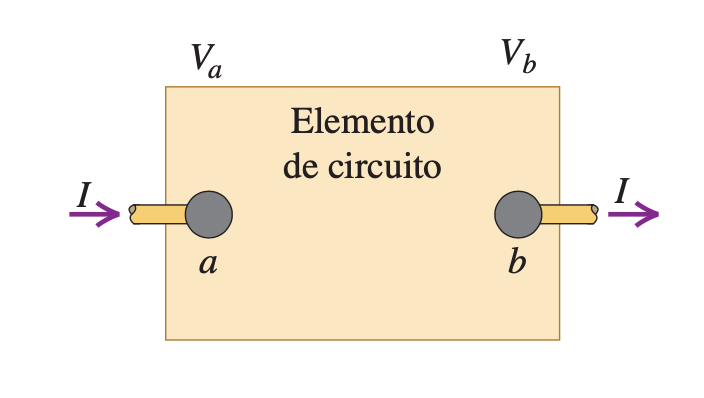
\includegraphics[scale=0.4]{fig/potencia}
\caption{La potencia de alimentación al elemento de circuito entre $a$ y $b$ es $P=(V_a-V_b)I=V_{ab}I$}
\label{fig:potencia}
\end{figure}

La caja de la figura \ref{fig:potencia} representa un elemento de circuito con diferencia de potencial $V_a-V_b=V_{ab}$ entre sus terminales y la corriente $I$ que pasa a través suyo en dirección de $a$ hacia $b$. Conforme la carga pasa por el elemento de circuito, el campo eléctrico realiza trabajo sobre la carga.

En los circuitos eléctricos es más frecuente que interese la \textit{rapidez} con la que la energía se proporciona a un elemento de circuito o se extrae de él. Si la corriente a través del elemento es $I$, entonces en un intervalo de tiempo $dt$ pasa una cantidad de carga $dQ=I\, dt$ a través del elemento. El cambio en la energía potencial para esta cantidad de carga es $V_{ab}\, dQ=V_{ab} I\, dt$.  Si esta expresión se divide entre $dt$, se obtiene la rapidez a la que se transfiere la energía hacia fuera o hacia dentro de circuito. La relación de transferencia de energía por unidad de tiempo es la \textit{potencia}, y se denota mediante $P$

\begin{equation}\label{25.17}\marginnote{Rapidez con la que se entrega energía a un elemento de circuito o se extrae de éste}
\boxed{P=V_{ab}I}
\end{equation}

\subsection{Potencia de una resistencia pura}
Si el elemento de circuito de la figura \ref{fig:potencia} es un resistor, la diferencia de potencial es $V_{ab}=IR$. De ecuación \ref{25.17}, la potencia eléctrica entregada al resistor por circuito es

\begin{equation}\label{25.18}\marginnote{Potencia entregada a un resistor}
P=V_{ab}I=I^2R=\frac{{V_{ab}}^2}{R}
\end{equation}














































